
\title{Error Correction in a Phenomenological Fibonacci Anyon Quantum Code}

\author{Simon Burton, Courtney Brell, Steven Flammia}
%\date{\today}

\documentclass[12pt,a4paper]{article}
%\documentclass[11pt, twocolumn]{article}

\usepackage[paper=a4paper,dvips,top=1.5cm,left=1.5cm,right=1.5cm,
    foot=1cm,bottom=1.5cm]{geometry}

%\usepackage{epsf}
\usepackage{amsmath}
\usepackage{color}
\usepackage{natbib}
%\usepackage{cite}

\RequirePackage{amsmath}
\RequirePackage{amssymb}
\RequirePackage{amsthm}
%\RequirePackage{algorithmic}
%\RequirePackage{algorithm}
%\RequirePackage{theorem}
%\RequirePackage{eucal}
\RequirePackage{color}
\RequirePackage{url}
\RequirePackage{mdwlist}

\RequirePackage[all]{xy}
\CompileMatrices
\RequirePackage{hyperref}
\RequirePackage{graphicx}
\RequirePackage[dvips]{geometry}


\begin{document}

\maketitle

\def\Complex {C}
\def\tensor{\otimes}
\def\Tensor{\bigotimes}
\def\bra #1{\langle #1|}
\def\ket #1{|#1\rangle}
\def\braket #1#2{\langle #1|#2 \rangle}

%\def\Set{\widetilde{\text{Set}}}
%\def\Top{\widetilde{\text{Top}}}
%\def\Vec{\widetilde{\text{Vec}}}
%\def\Chain{\widetilde{\text{Chain}}}

%\def\ker{\text{ker}}
%\def\coker{\text{coker}}
%\def\im{\text{im}}

%\def\H{\mathcal{H}}
%\def\H{H}
%\def\S{S}
\def\mathZ{\mathbb{Z}}
\def\mathR{\mathbb{R}}

%\def\nin{\not\in}


% ----------------------------------------------------------------------------
%

\section{Braid group}

Braid group on $n$ strands is the group $B_n$ generated by $n-1$ generators
$\sigma_1, \sigma_2, ... \sigma_{n-1}$ with the following relations:
    $$ \sigma_i \sigma_j = \sigma_j \sigma_i \ \text{when}\ |i-j| > 2, $$
    $$ \sigma_i \sigma_{i+1} \sigma_i =  \sigma_{i+1} \sigma_i \sigma_{i+1}.$$


% ----------------------------------------------------------------------------

\section{Fibonacci Anyons}


So we have a (linear) representation of the braid group.


% ----------------------------------------------------------------------------

\section{Curve Diagrams}


Given a topological space $X$ we define the {\it mapping class group} of $X$ as
the set of homeomorphisms $f:X\to X$ modulo isotopy

    % $$ MCG(X) := \{ f : X \to X \text{s.t.} f \text{is homeomorphism} \} / \sim_{\text{iso}} $$
    $$ MCG(X) := \{ f : X \to X \} / \sim_{\text{iso}}.$$


In particular we are interested in the $n$-punctured disc:

    $$ D_n := \mathR^2 - Q_n.$$

topologically this is a sphere with $n+1$ holes in it.

It is a theorem that the group $MCG(D_n)$ is isomorphic to $B_n.$
(See \cite{Kassel10}, chapter 1.)

Curve diagrams, see \cite{Dehornoy02}.

We verify the braid relations directly.


\begin{center}
%\includegraphics[width=0.5\textwidth]{mypicture.png}
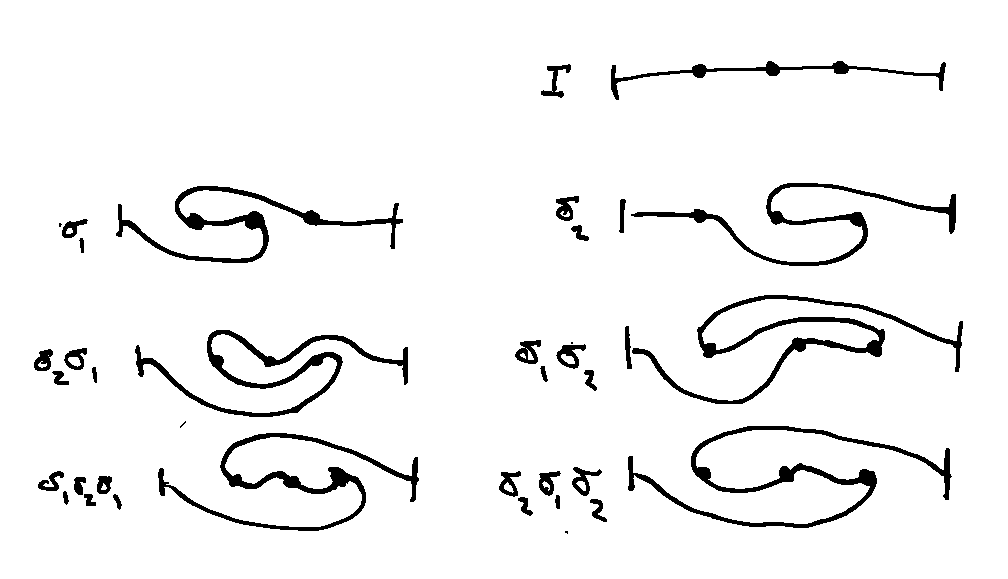
\includegraphics{curve-braid.eps}
\end{center}



% ----------------------------------------------------------------------------

\bibliography{refs}{}
\bibliographystyle{abbrv}

\end{document}


